% scrreprt ist eine verbesserte Version von report
\documentclass[11pt]{scrreprt} 



%%%%%%%%%%%%%%%%%%%%%%%%%%%%%%%%%%%%%%%%%%%%%%%%%%
% Paket zum sezten der Papiergroesse und Raendern
\usepackage{vmargin}
\setpapersize[landscape]{A3} % aus vmargin
%\setmarginsrb{leftmargin}{topmargin}{rightmargin}{bottommargin}{headheight}{headsep}{footheight}{footskip}
\setmarginsrb{23.0cm}{1.8cm}{2.5cm}{2.3cm}{\baselineskip}{0.9cm}{1.1cm}{1.4cm}

%%%%%%%%%%%%%%%%%%%%%%%%%%%%%%%%%%%%%%%%%%%%%%%%%%
% Einbinden von Bildern
\usepackage{graphicx}
\usepackage{epstopdf}
\usepackage{setspace}


%%%%%%%%%%%%%%%%%%%%%%%%%%%%%%%%%%%%%%%%%%%%%%%%%%
%\usepackage[ansinew]{inputenc}
\usepackage[T1]{fontenc}
\usepackage[utf8]{inputenc}
%\usepackage{ae}

%%%%%%%%%%%%%%%%%%%%%%%%%%%%%%%%%%%%%%%%%%%%%%%%%%
% drehen von Text, wird für die beschriftung des 
% Buchrueckens benoetigt
\usepackage{rotating}

\begin{document}
\graphicspath{{./Pictures/}}


% Titelseite
\begin{titlepage}
\setlength{\voffset}{-.5 cm}
%\begin{flushright}
%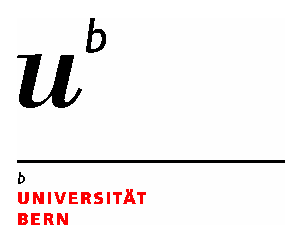
\includegraphics[scale=0.3, trim= 40mm 1mm 5mm 20mm]{logo} \\[1.8 cm]
%\end{flushright}
\begin{center}

\begin{spacing}{2.5}
{\Huge \bfseries Characterization of the Pre-Lytic Active Egress of a Non-Enveloped Virus} \\[3.5 cm]
\end{spacing}
{\Large Inauguraldissertation \\
der Philosophisch-naturwissenschaftlichen Fakultät \\
der Universität Bern \\[2.5cm]
{\large vorgelegt von}\\[0.3 cm]
{\LARGE \textbf{\textsc{Raphael Wolfisberg}}} \\[0.3 cm] 
{\large von Neuenkirch, LU} \\ [2.5 cm]
{\Large Leiter der Arbeit:\\ [0.5 cm]
{\textsc Prof. Dr. Christoph Kempf} \\
and \\
{\textsc PD Dr. Carlos Ros} \\ [1.3 cm]
Departement für Chemie und Biochemie}}
\end{center}

      %%%%%%%%%%%%%%%%%%%%%%%%%%%%%%%%%%%%%%%%%%%%%%%%%%% 
      % Buchruecken beschriften     
      \begin{picture}(0,0)      
        \put(-110,110){\begin{sideways}{\LARGE\textbf{Characterization of the Pre-Lytic Active Egress of a Non-Enveloped Virus}}\end{sideways}}
        \put(-110,-75){\begin{sideways}{\LARGE\textbf{Raphael Wolfisberg}}\end{sideways}}
      \end{picture}     
      %%%%%%%%%%%%%%%%%%%%%%%%%%%%%%%%%%%%%%%%%%%%%%%%%%% 

\end{titlepage}



\end{document}



